\documentclass{standalone}
\usepackage{tikz}
\usetikzlibrary{shapes.geometric, arrows, positioning}

\begin{document} 
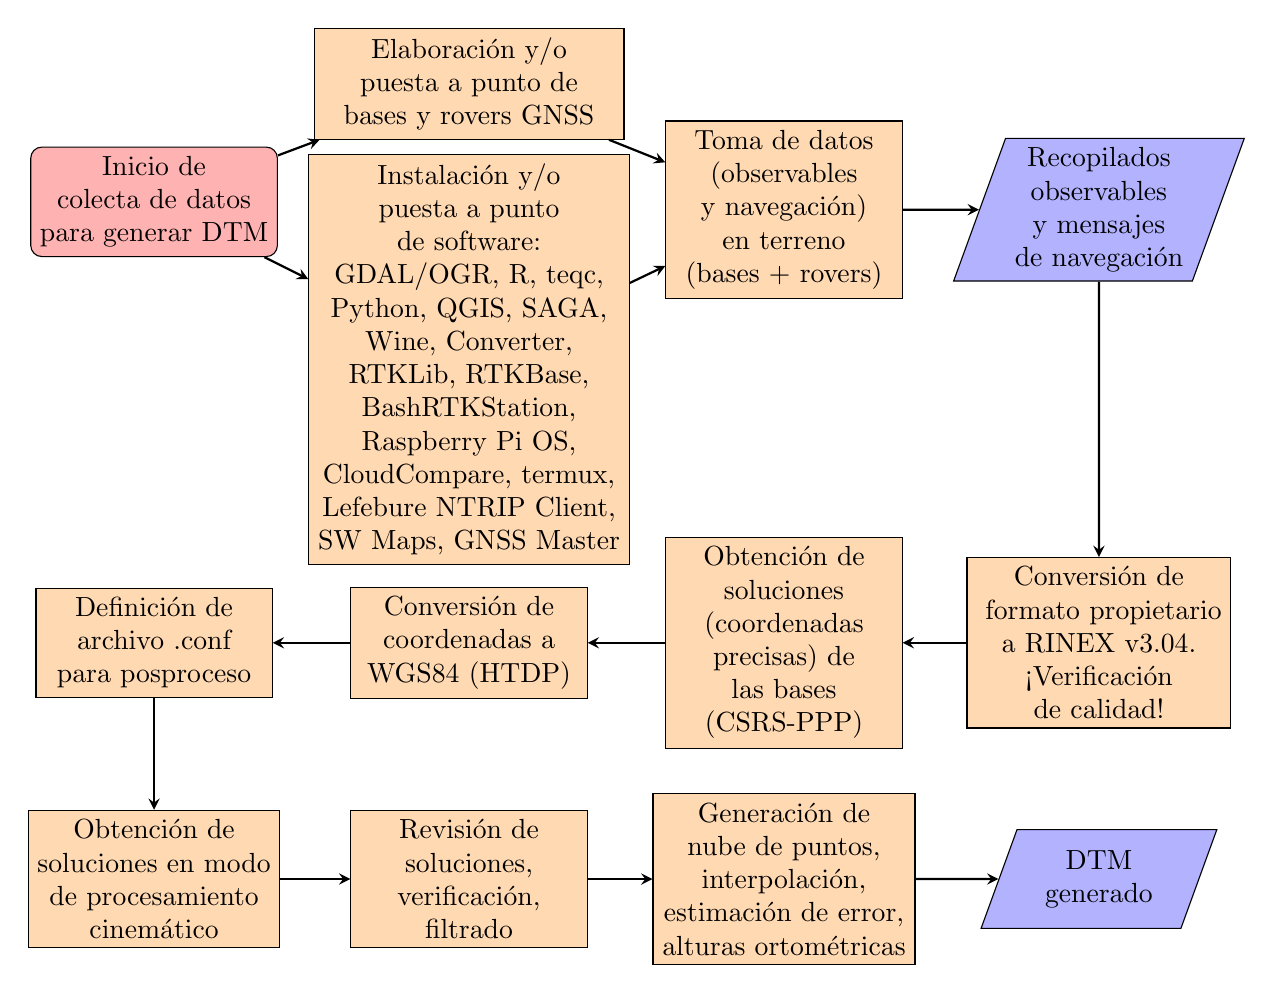
\begin{tikzpicture}[
  startstop/.style={rectangle, rounded corners, minimum width=3cm, minimum height=1cm,text centered, align=center, draw=black, fill=red!30},
  io/.style={trapezium, trapezium left angle=70, trapezium right angle=110, minimum width=3cm, minimum height=1cm, text centered, align=center, draw=black, fill=blue!30},
  process/.style={rectangle, minimum width=3cm, minimum height=1cm, text centered, align=center, draw=black, fill=orange!30},
  decision/.style={diamond, minimum width=3cm, minimum height=1cm, text centered, align=center, draw=black, fill=green!30},
  arrow/.style={thick,->,>=stealth}]

  % Nodes
  \node (start) [startstop] {Inicio de \\ colecta de datos \\ para generar DTM};
  \node (bases) [process, right of=start, yshift=1.5cm, xshift=3cm] {Elaboración y/o \\ \,\,\,\,\,\,\,\,puesta a punto de\,\,\,\,\,\,\,\, \\ bases y rovers GNSS};
  \node (software) [process, right of=start, yshift=-2cm, xshift=3cm] {Instalación y/o \\ puesta a punto \\ de software: \\ GDAL/OGR, R, teqc, \\ Python, QGIS, SAGA, \\ Wine, Converter,\\ RTKLib, RTKBase, \\ BashRTKStation, \\ Raspberry Pi OS, \\ CloudCompare, termux, \\ Lefebure NTRIP Client, \\ SW Maps, GNSS Master};
  \node (tomadatos) [process, right of=bases, yshift=-1.6cm, xshift=3cm] {Toma de datos \\ (observables \\ y navegación) \\ en terreno \\ (bases + rovers)};
  \node (datostomados) [io, right of=tomadatos, xshift=3cm] {Recopilados \\ observables \\ y mensajes \\ de navegación};
  \node (conversion) [process, below of=datostomados, yshift=-4.5cm] {Conversión de \\\ formato propietario \\ a RINEX v3.04. \\ ¡Verificación \\ de calidad!};
  \node (pppbases) [process, left of=conversion, xshift=-3cm] {Obtención de \\ soluciones \\ (coordenadas \\ precisas) de \\ las bases \\ (CSRS-PPP)};
  \node (conversionwgs84) [process, left of=pppbases, xshift=-3cm] {Conversión de \\ coordenadas a \\ WGS84 (HTDP) };
  \node (archivoconf) [process, left of=conversionwgs84, xshift=-3cm] {Definición de \\ archivo .conf \\ para posproceso};

  \node (posproceso) [process, below of=archivoconf, yshift=-2cm] {Obtención de \\ soluciones en modo \\ de procesamiento \\ cinemático};
  \node (revision) [process, right of=posproceso, xshift=3cm] {Revisión de \\ soluciones, \\ verificación, \\ filtrado};
  \node (nubedepuntos) [process, right of=revision, xshift=3cm] {Generación de \\ nube de puntos,\\ interpolación, \\ estimación de error, \\ alturas ortométricas};
  \node (end) [io, right of=nubedepuntos, xshift=3cm] {DTM \\ generado};

  % Arrows
  \draw [arrow] (start) -- (bases);
  \draw [arrow] (start) -- (software);
  \draw [arrow] (bases) -- (tomadatos);
  \draw [arrow] (software) -- (tomadatos);
  \draw [arrow] (tomadatos) -- (datostomados);

  \draw [arrow] (datostomados) -- (conversion);
  \draw [arrow] (conversion) -- (pppbases);
  \draw [arrow] (pppbases) -- (conversionwgs84);
  \draw [arrow] (conversionwgs84) -- (archivoconf);

  \draw [arrow] (archivoconf) -- (posproceso);
  \draw [arrow] (posproceso) -- (revision);
  \draw [arrow] (revision) -- (nubedepuntos);
  \draw [arrow] (nubedepuntos) -- (end);
  
\end{tikzpicture}
\end{document}
